\documentclass[UTF8]{ctexbeamer}	% Compile at least twice!
%\setbeamertemplate{navigation symbols}{}
\usetheme{Antibes}
% \useinnertheme{rectangles}
\useoutertheme{infolines}
\useoutertheme[title,section,subsection=true]{smoothbars}
% \useoutertheme{split}
\useinnertheme{rounded}
\usecolortheme{default}
% \usecolortheme{whale}
 
% -------------------
% Packages
% -------------------
\usepackage{
    amsmath,			% Math Environments
    amssymb,			% Extended Symbols
    enumerate,		    % Enumerate Environments
    graphicx,			% Include Images
    lastpage,			% Reference Lastpage
    multicol,			% Use Multi-columns
    multirow,			% Use Multi-rows
    pifont,			    % For Checkmarks
    stmaryrd,            % For brackets
    listings,
}
\usepackage[english]{babel}
\usepackage{graphicx}
% \usepackage{CJK}
\lstset{language=C++}
\lstset{extendedchars=false}
\lstset{breaklines}


% -------------------
% Colors
% -------------------
% \definecolor{UniOrange}{RGB}{212,69,0}
% \definecolor{UniGray}{RGB}{62,61,60}
% \definecolor{UniRed}{HTML}{B31B1B}
% \definecolor{UniGray}{HTML}{222222}
% \setbeamercolor{title}{fg=UniGray}
% \setbeamercolor{frametitle}{fg=UniOrange}
% \setbeamercolor{structure}{fg=UniOrange}
% \setbeamercolor{section in head/foot}{bg=UniGray}
% \setbeamercolor{author in head/foot}{bg=UniGray}
% \setbeamercolor{date in head/foot}{fg=UniGray}
% \setbeamercolor{structure}{fg=UniOrange}
% \setbeamercolor{local structure}{fg=black}
% \beamersetuncovermixins{\opaqueness<1>{0}}{\opaqueness<2->{15}}


% -------------------
% Fonts & Layout
% -------------------
\useinnertheme{default}
\usefonttheme{serif}
\usepackage{palatino}
\setbeamerfont{title like}{shape=\scshape}
\setbeamerfont{frametitle}{shape=\scshape}
\setbeamertemplate{itemize items}[circle]
%\setbeamertemplate{enumerate items}[default]


% -------------------
% Commands
% -------------------

% Special Characters
\newcommand{\N}{\mathbb{N}}
\newcommand{\Z}{\mathbb{Z}}
\newcommand{\Q}{\mathbb{Q}}
\newcommand{\R}{\mathbb{R}}
%\newcommand{\C}{\mathbb{C}}

% Math Operators
\DeclareMathOperator{\im}{im}
\DeclareMathOperator{\Span}{span}

% Special Commands
\newcommand{\pf}{\noindent\emph{Proof. }}
\newcommand{\ds}{\displaystyle}
\newcommand{\defeq}{\stackrel{\text{def}}{=}}
\newcommand{\ov}[1]{\overline{#1}}
\newcommand{\ma}[1]{\stackrel{#1}{\longrightarrow}}
\newcommand{\twomatrix}[4]{\begin{pmatrix} #1 & #2 \ #3 & #4 \end{pmatrix}}


% -------------------
% Tikz & PGF
% -------------------
\usepackage{tikz}
\usepackage{tikz-cd}
\usetikzlibrary{
    calc,
    decorations.pathmorphing,
    matrix,arrows,
    positioning,
    shapes.geometric
}
\usepackage{pgfplots}
\pgfplotsset{compat=newest}

\usepackage{wrapfig}
\usepackage{cite}


% -------------------
% Theorem Environments
% -------------------
\theoremstyle{plain}
\newtheorem{sit}{Situation}[section]
\newtheorem{prop}{Proposition}[section]
\newtheorem{rtm}{Theorem}[section]
\newtheorem{cor}{Corollary}[section]
\theoremstyle{definition}
\newtheorem{das}{Data structure}[section]
\newtheorem{nex}{Non-Example}[section]
\newtheorem{cla}{class}[section]
\newtheorem{emt}{}[section]
\newtheorem{defn}{Definition}[section]
\theoremstyle{remark}
\newtheorem{rem}{Remark}[section] 
\numberwithin{equation}{section}

\newcommand\caesura{$\mkern -8.5mu\raise -.2ex\hbox{\rotatebox[]{180}{\`}}\ $}

% -------------------
% Title Page
% -------------------
\title{\textcolor{white}{2022年硕博连读综合面试报告}}
%\subtitle{\textcolor{white}{Mathematics Conference for the Mysterious and dMagical}}  
\author{谭焱(张庆海)}
\institute{浙江大学数学科学学院}
\date{\today} 


% -------------------
% Content
% -------------------
\begin{document}
% \begin{CJK}{GBK}{kai}

% Title Page
\begin{frame}
\titlepage
\end{frame}



% Motivation
\section{个人基本情况介绍}


% \begin{frame}
%     \begin{emt}[过往受教育经历]
%         \begin{enumerate}
%             \item 高中在湖南师范大学附属中学就读时参与数学奥林匹克竞赛.
%         \end{enumerate}
        
%     \end{emt}
% \end{frame}


% Definitions & Examples
\begin{frame}[fragile]
    \begin{emt}[个人学习经历]
\begin{enumerate}
    \item 高中在湖南师大附中就读时参与数学奥林匹克竞赛.
    \begin{itemize}
        \item 高二高三两年获得数学竞赛省一等奖.
    \end{itemize}
    \item 研究生课程学分修读情况
    \begin{itemize}
        \item 已修满硕士学位要求的学分,并在与我的科研项目相关的部分课程中取得良好成绩.
        \begin{itemize}
            \item 非线性问题的数学方法(92), 图形学的新进展(90) 等.
        \end{itemize}
        \item 英语阅读及写作方面
        \begin{itemize}
            \item 六级489分(阅读205)可以流畅阅读英文文献.
            \item 通过课程研究生论文写作指导(92)打下坚实写作基础.
        \end{itemize}
    \end{itemize}
\end{enumerate}
\end{emt}
\end{frame}

\begin{frame}[fragile]
   \begin{emt} [研究生项目参与情况]
    \begin{enumerate}
        \item 2019年春学期,独立完成程序.实现张老师的论文中的二维空间内殷集上的布尔代数.
        为之后的三维空间内殷集之间的布尔代数的研究做好铺垫.
        % 
\includegraphics[width = \linewidth]{fig/articlename1.png}
        \item 2020年秋学期,在张老师的指导下,和学长合作完成项目微地震反问题.最终得到一个能根据
        检波器接收到的地震波信号输出合理的震源位置的程序.
        \item 2021年春学期,与学弟分工推进三维殷集的表示,及通过编程实现在计算机上计算
        三维殷集之间的布尔运算.
    \end{enumerate}
   \end{emt}
\end{frame}

\section{研究生项目详细介绍}
\subsection{微地震的反问题}

\begin{frame}
    \frametitle{微地震探测反问题研究}
    \begin{itemize}
        \setlength{\itemsep}{30pt}
        \item \textbf{背景 : } 项目的意义和要做的问题.
        \item  \textbf{解决过程 : } 切分问题,分步实现.
        \item \textbf{实现结果 : } 对真实数据计算结果图和总结.
    \end{itemize}
\end{frame}

\begin{frame}
    \begin{emt}[背景及意义]
      
    \begin{itemize}
        \begin{columns}
            \column{0.8\linewidth}<1->
    % \begin{wrapfigure}[r]{5cm}
    %    \centering
    %    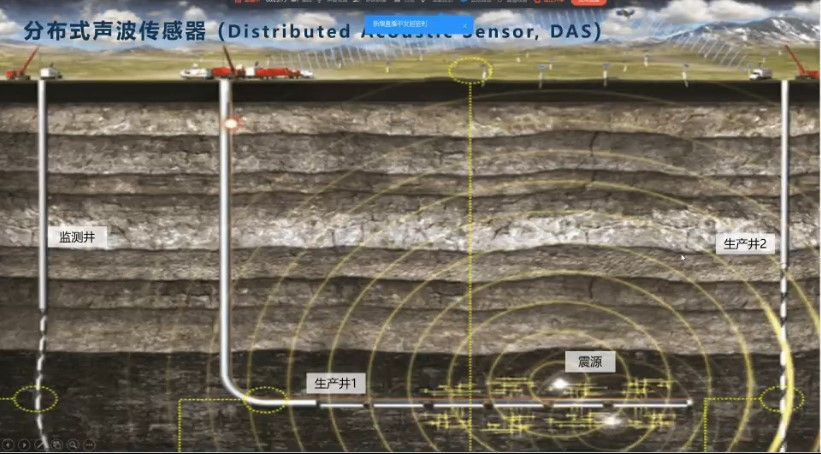
\includegraphics[width = \textwidth]{fig/s2p1.jpg}
    %    \caption{\footnote{ 油气田中的生产井和监测井}}
    % \end{wrapfigure}
    \column{0.2\linewidth}<1->
    \item  微地震通常是由于地质勘探或者一些开采活动导致地下裂缝错位,从而形成的
低频率弹性波.\cite{wu_1991}
\end{columns}
\item 作为一种人为产生的地震,其产生的信号可以用于石油工程作业.
近些年来,国际上众多的研究机构与微震公司已经证明了微地震监测方法在油气田
规划与开发方面的指导意义.

    \end{itemize}

    
\end{emt}
\end{frame}


% \end{CJK}
\end{document}